%\documentclass{report}
%\usepackage[T1]{fontenc}
%\usepackage[utf8]{inputenc}
%\usepackage[francais]{babel}
%\usepackage{amsmath}
%\usepackage{graphicx}
%\graphicspath{{Figures/}}
%\usepackage[backend=biber,style=authoryear,bibencoding=utf8]{biblatex}
%\usepackage[colorlinks,linkcolor=blue]{hyperref}
%\newcommand{\micro}{$\mathrm{\mu}$}
%
%\begin{document}

\chapter{Localisation de MRTF-A dans les cellules musculaires en réponse à une stimulation mécanique}

\section{À propos de la localisation de MRTF-A}

\section{Application d'une force locale avec les pinces magnétiques}

Pour réaliser des expériences sur les cellules transfectées MRTF-A GFP, il a fallu monter les pinces magnétiques sous le microscope confocal. 
L'observation se faisait avec un objectif 40X à air, dans la géométrie à courte distance, ce qui nous permet d'appliquer localement de grandes forces (plusieurs centaines de pN) mais nous empêche d'observer suffisamment bien la position de la bille pour faire des mesures rhéologiques. 
Dans un premier temps, l'objectif était simplement de voir si l'application d'une force par les pinces magnétiques était suffisante pour déclencher une relocalisation de MRTF-A dans les cellules musculaires. 

Nous avons réalisé ces expériences sur trois séries de C2C12 : transfectées avec MRTF-A GFP seule (37 cellules observées), tranfectées avec MRTF-A GFP et une Actine mCherry (16 cellules observées), et transfectées avec MRTF-A GFP et le LifeAct RFP, qui marque les filaments d'actine dans les cellules vivantes (42 cellules observées, dont 34 témoins). 
L'objectf de ces doubles transfections était d'observer en même temps que la localisation de MRTF-A la réorganisation du cytosquelette. 

Parmi ces expériences, certaines cellules ont été observées alors qu'elles n'avaient pas de bille attachée à leur cytosquelette : ce sont des cellules témoins, sur lesquelles le champ magnétique a été appliqué comme pour les autres, mais sur lesquelles le champ n'est pas censé avoir un effet quelconque. 

\begin{figure}
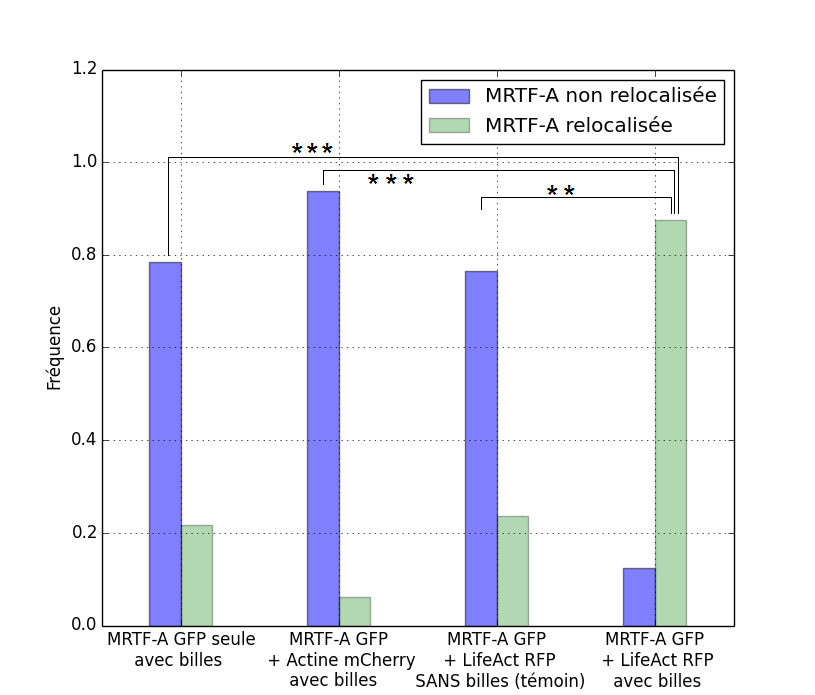
\includegraphics[scale=0.5]{Figures/Pinces_MRTFA_stars.png} 
\caption{Proportion des cellules observées pour lesquelles MRTF-A GFP change (en vert) ou ne change pas (en bleu) de localisation dans la cellule au cours de l'expérience. * : p<0.05 , ** p<0.01, *** p<0.001 (réalisés avec un test de Fisher)\label{MRTF-A Pinces}}
\end{figure}

On peut voir sur la figure \ref{MRTF-A Pinces} que l'ajout d'actine exogène réduit le nombre de cellules pour lesquelles MRTF-A change de localisation, mais de manière non significative, alors que l'ajout de Life Act RFP a l'effet inverse de manière significative. 
En effet, en ajoutant de l'actine mCherry, on augmente la quantité totale de G-actine dans la cellule, et ce d'autant plus que l'actine fluorescente polymérise un peu moins bien que l'actine sauvage. Comme plus de G-actine est disponible pour se lier à MRTF-A, celle-ci est d'autant plus susceptible d'être liée à l'actine et donc cytoplasmique. 
Si la réserve d'actine monomérique est grande, une polymérisation d'actine en réponse à la force appliquée ne sera pas forcément suffisante pour dépléter la réserve de G-actine excédentaire.

Au contraire, la LifeAct, en se liant aux filaments d'actine, peut les stabiliser en conformation polymérisée. En stabilisant la F-actine, la LifeAct rend donc la cellule beaucoup plus sensible à un recrutement de G-actine pour former de nouveaux filaments, et MRTF-A est plus susceptible de se retrouver sans liaison avec l'actine, et donc nucléaire.

De plus, on peut voir en comparant avec les expériences LifeAct témoin sans bille que l'application d'une force sur la cellule a un effet significatif sur la relocalisation de MRTF-A. 

On peut également remarquer que les résultats pour MRTF-A GFP seule sont identiques aux résultats avec LifeAct RFP mais sans application de force. 
On peut raisonnablement supposer que la force appliquée n'est pas suffisante ou n'est pas appliquée suffisamment longtemps pour réorganiser significativement le cytosquelette lors des expériences MRTF-A GFP seule, ce qui explique que leur activité soit proche des cellules témoins. 
La présence de Life-Act RFP stabilisant les filaments, la réserve d'actine monomérique est plus faible dans les cellules doublement transfectées MRTF-A GFP + LifeAct RFP, ce qui les rend plus sensibles : une contrainte plus faible suffit à dépléter suffisamment la réserve de G-actine. 



























%\end{document}